\documentclass[aspectratio=169]{beamer}
\usetheme{Madrid}
\usepackage{booktabs}
\usepackage{graphicx}
\usepackage{array}

\title{Branch Specialization Checkpoint}
\subtitle{Toy Competition Layout Permutations}
\author{Branch Specialization Project}
\date{2026-05-22}

\begin{document}

\begin{frame}
  \titlepage
  \vspace{-0.5em}
  \begin{center}
    Checkpoint reason: new result refines the Phase 3 architectural-intervention claim.
  \end{center}
\end{frame}

\begin{frame}{Current Question}
  \textbf{Phase 3 RQ:} Does structural heterogeneity cause more stable functional specialization?

  \vspace{1em}
  After the local-vs-induction competition result, the sharper question is:

  \vspace{0.5em}
  \begin{quote}
    When the 64-dim head is moved to each possible head position, do functions follow
    dimension, index, or broader layout?
  \end{quote}

  \vspace{0.5em}
  This tests whether heterogeneous head dimensions create semantic role classes, or
  just break permutation symmetry by making stable capacity slots.
\end{frame}

\begin{frame}{Experiment Setup}
  \begin{itemize}
    \item Task combines local copy and induction-style continuation in one sequence.
    \item Local region: \texttt{[x, SEP, x]}, scored at \texttt{SEP}.
    \item Induction region: \texttt{[y1, ..., y16, y1, ..., y16]}, scored on second-half continuation.
    \item Same total attention dimension: 128.
    \item Five seeds per layout, 1200 training steps per seed.
    \item Role score is causal single-head ablation loss delta.
  \end{itemize}

  \vspace{0.5em}
  \[
  S_r(h) = \max(\mathrm{loss}_r(\mathrm{ablate}\ h) - \mathrm{loss}_r(\mathrm{base}), 0)
  \]
\end{frame}

\begin{frame}{Layouts Tested}
  \begin{center}
  \small
  \begin{tabular}{llcc}
    \toprule
    Config & Head dimensions & Local acc. & Induction acc. \\
    \midrule
    \texttt{hetero4\_64first} & [64, 16, 16, 32] & 0.9999 & 0.9986 \\
    \texttt{hetero4\_64second} & [16, 64, 16, 32] & 1.0000 & 1.0000 \\
    \texttt{hetero4\_64third} & [16, 32, 64, 16] & 1.0000 & 0.9993 \\
    \texttt{hetero4} & [16, 16, 32, 64] & 1.0000 & 0.9992 \\
    \bottomrule
  \end{tabular}
  \end{center}

  \vspace{0.7em}
  All layouts learn both objectives, so the slot pattern is not a failure-to-learn artifact.
\end{frame}

\begin{frame}{Main Evidence}
  \begin{center}
  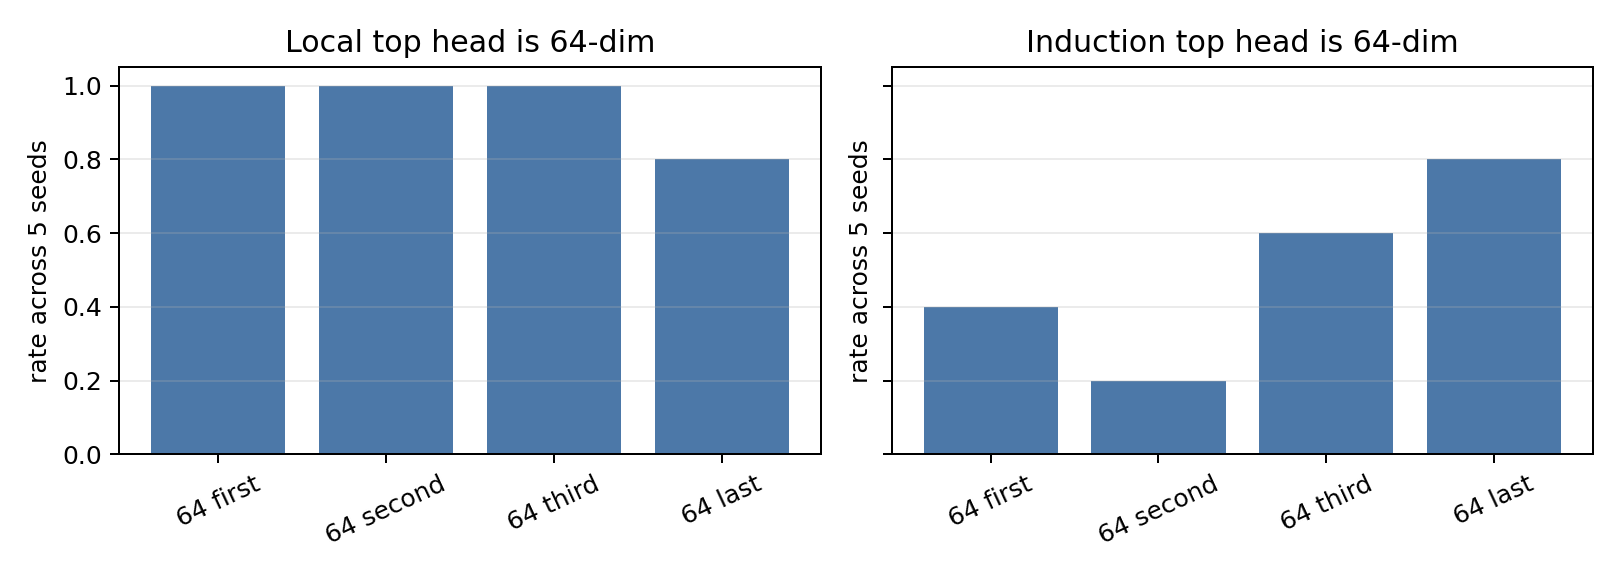
\includegraphics[width=0.86\linewidth]{figures/top_64_rate_by_layout.png}
  \end{center}

  \vspace{-0.4em}
  \begin{itemize}
    \item Local role almost always occupies the 64-dim head.
    \item Induction role is layout-sensitive and only uses the 64-dim head in half of runs.
  \end{itemize}
\end{frame}

\begin{frame}{Aggregate Result}
  \begin{center}
  \small
  \begin{tabular}{lrrrr}
    \toprule
    Role & Models & Top head 64-dim & Mean top spec. & Mean top loss delta \\
    \midrule
    Local & 20 & 19/20 & 0.9180 & 0.1457 \\
    Induction & 20 & 10/20 & 0.7388 & 2.5272 \\
    \bottomrule
  \end{tabular}
  \end{center}

  \vspace{1em}
  The local role follows the 64-dim head across positions H0, H1, H2, and H3.
  Induction splits evenly between 64-dim and 16-dim top slots.
\end{frame}

\begin{frame}{Interpretation}
  \textbf{Supported:}
  \begin{itemize}
    \item Heterogeneous head dimensions create stable high-capacity slots.
    \item The local/previous-token role strongly prefers the 64-dim slot.
    \item The function-to-slot mapping is much more stable than uniform 4-head baselines.
  \end{itemize}

  \vspace{0.7em}
  \textbf{Not supported:}
  \begin{itemize}
    \item A simple semantic taxonomy where small heads become local and large heads become induction/global.
    \item Dimension alone determining role assignment.
  \end{itemize}
\end{frame}

\begin{frame}{Decision}
  Narrow the Stage 3 claim:

  \vspace{0.8em}
  \begin{quote}
    Structural heterogeneity can stabilize function-to-slot mappings by breaking
    permutation symmetry, but task pressure and layout mediate which function gets
    each slot.
  \end{quote}

  \vspace{0.8em}
  Next decisive experiment:
  \begin{enumerate}
    \item Sweep local-vs-induction objective weights on the same task.
    \item Test whether reducing local pressure lets induction occupy the 64-dim slot more often.
    \item If roles flip with weights, frame the mechanism as capacity-slot competition.
  \end{enumerate}
\end{frame}

\begin{frame}{Sources and Provenance}
  \scriptsize
  \begin{itemize}
    \item Report: \texttt{doc/phase3\_toy\_competition\_layout\_permutations.md}
    \item Training script: \texttt{scripts/toy\_competition\_head\_dim\_intervention.py}
    \item Analysis script: \texttt{scripts/analyze\_competition\_layout\_permutations.py}
    \item New run: \texttt{results/phase3\_toy\_competition\_layout\_permutations/}
    \item Combined analysis: \texttt{results/phase3\_toy\_competition\_layout\_analysis/}
    \item Deck data snapshot: \texttt{presentations/2026-05-22-0858-layout-permutation/data/}
  \end{itemize}
\end{frame}

\end{document}
